\documentclass[tikz, border=0px]{standalone}
\usepackage{tikz}
\usetikzlibrary{shapes,arrows}

\tikzstyle{startstop} = [rectangle,rounded corners,minimum width=3cm,minimum height=1cm,align=center,draw=black, text width=2.5cm, fill=green!30]

\tikzstyle{therapy} = [trapezium, trapezium left angle =70, trapezium right angle=110, minimum width=2cm, minimum height = 1cm, centered,draw=black,align=center, text width=2cm, fill=orange!30]

\tikzstyle{decision} = [diamond, minimum width = 3cm, minimum height = 3cm, text centered, draw=black, text width = 2cm,align=center,fill=blue!30]

\tikzstyle{arrow} = [thick, ->, >=stealth]
\tikzstyle{doublearrow} = [<->, thick, >=stealth]

\begin{document}
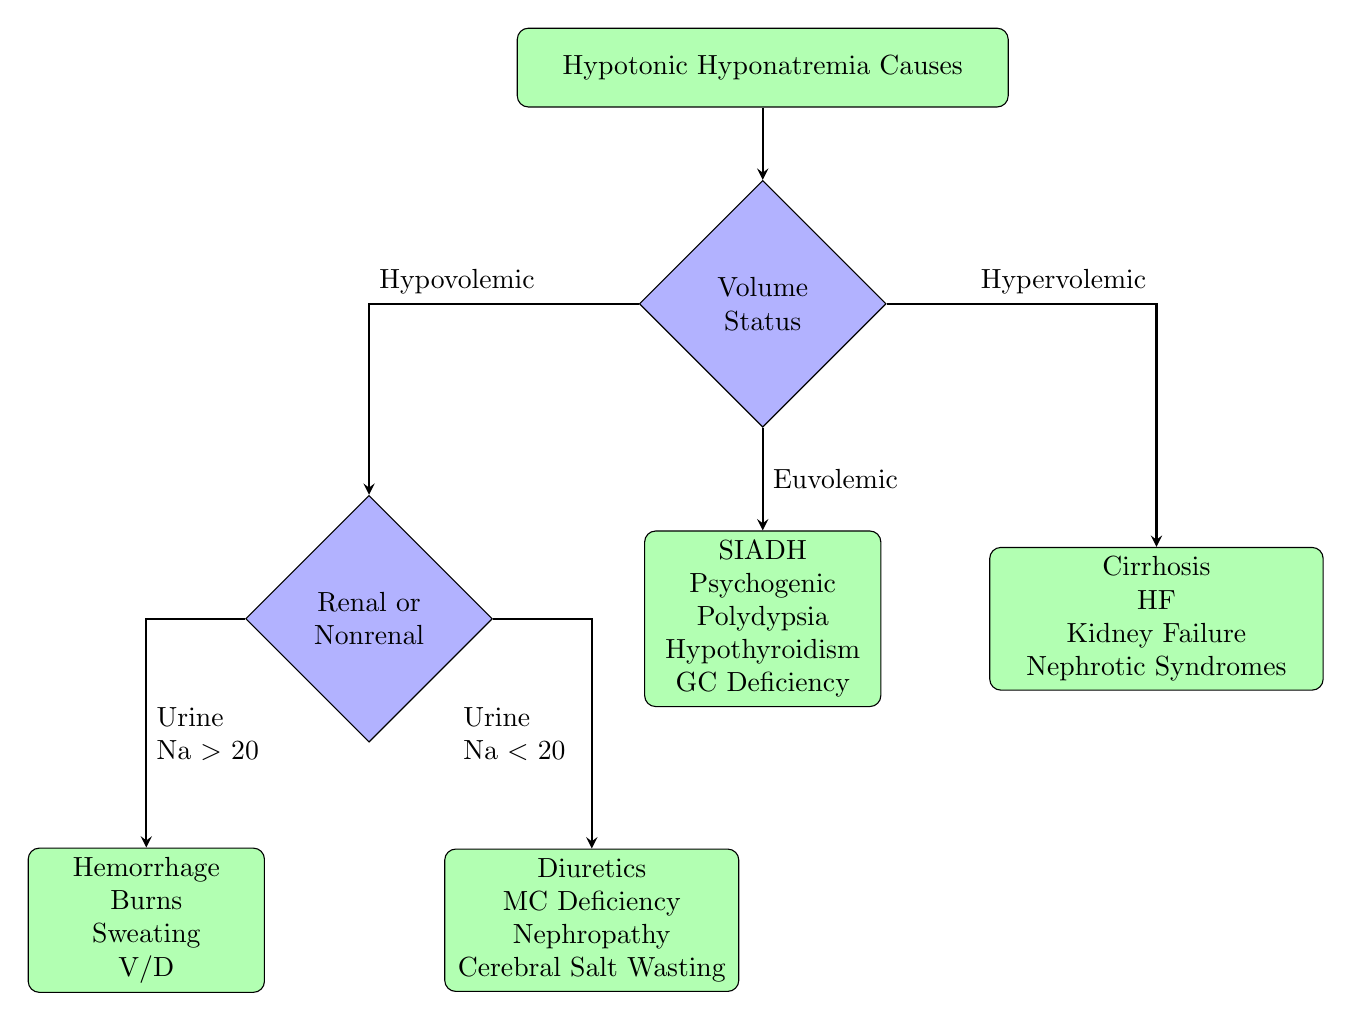
\begin{tikzpicture}[node distance=4cm]

\node (start) [startstop, text width = 6cm] {Hypotonic Hyponatremia Causes};
\node (volStat) [decision, below of=start,yshift=1cm] {Volume Status};
\node (hypoVol) [decision, below of=volStat, xshift=-5cm] {Renal or Nonrenal};
\node (nonRenal) [startstop, below left of=hypoVol, yshift=-1cm] {Hemorrhage\\ Burns\\ Sweating\\ V/D};
\node (renal) [startstop, below right of=hypoVol, yshift=-1cm, text width = 3.5cm] {Diuretics\\ MC Deficiency\\ Nephropathy\\ Cerebral Salt Wasting};
\node (euVol) [startstop, below of=volStat] {SIADH\\ Psychogenic Polydypsia\\ Hypothyroidism\\ GC Deficiency};
\node (hyperVol) [startstop, below of=volStat, xshift=5cm,text width =4cm] {Cirrhosis\\ HF\\ Kidney Failure\\ Nephrotic Syndromes};

\draw [arrow] (start) -- (volStat);
\draw [arrow] (volStat) -| node [above right] {Hypovolemic} (hypoVol);
\draw [arrow] (volStat) -- node [right] {Euvolemic} (euVol);
\draw [arrow] (volStat) -| node [above left] {Hypervolemic} (hyperVol);
\draw [arrow] (hypoVol) -| node[below right, yshift = -1cm, text width = 1.5cm] {Urine\\Na $>$ 20} (nonRenal);
\draw [arrow] (hypoVol) -| node[below left, yshift = -1cm, text width = 1.5cm] {Urine\\Na $<$ 20} (renal);

\end{tikzpicture}
\end{document}